% !TeX encoding = UTF-8
% !TeX spellcheck = en_GB
% !TeX root = mythesis.tex
\chapter{Dilution cryostat wiring}

%The  Second appendix

\begin{figure}[hptb]
	\begin{center}
		\begin{tabular}{c}
			(a) \\ 
			
			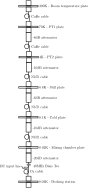
\includegraphics[height = 12 cm]{./appB/input_RF_line} 
		\end{tabular}
	\end{center}
	
	\caption{Input RF lines}
	\label{fig: Input RF lines}
\end{figure}

\begin{figure}[hptb]
	\begin{center}
		\begin{tabular}{c}
			(a) \\ 
			
			 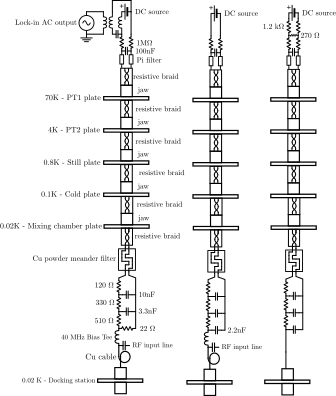
\includegraphics[height = 12 cm]{./appB/input_DC_line}
		\end{tabular}
	\end{center}
	
	\caption{Input DC lines}
	\label{fig: Input DC lines}
\end{figure}

\begin{figure}[hptb]
	\begin{center}
		\begin{tabular}{c}
			(a) \\ 
			
			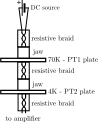
\includegraphics[height = 4 cm]{./appB/power_supply_ampli}
		\end{tabular}
	\end{center}
	
	\caption{amplifier supply lines}
	\label{fig: amplifier supply lines}
\end{figure}


\begin{figure}[hptb]
	\begin{center}
		\begin{tabular}{c}
			(a) \\ 
			
			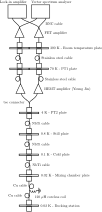
\includegraphics[height = 12 cm]{./appB/output_LF_line}
		\end{tabular}
	\end{center}
	
	\caption{output LF line}
	\label{fig: output LF line}
\end{figure}

\begin{figure}[hptb]
	\begin{center}
		\begin{tabular}{c}
			(a) \\ 
			
			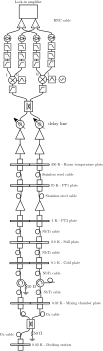
\includegraphics[height = 18 cm]{./appB/output_RF_noise_line}
		\end{tabular}
	\end{center}
	
	\caption{output RF noise line}
	\label{fig: output RF noise line}
\end{figure}

\begin{figure}[hptb]
	\begin{center}
		\begin{tabular}{c}
			(a) \\ 
			
			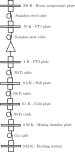
\includegraphics[height = 12 cm]{./appB/output_RF_current_line}
		\end{tabular}
	\end{center}
	
	\caption{output RF current line}
	\label{fig: output RF current line}
\end{figure}

\eqref{eq: RF power after one attenuator}
\begin{equation}
P_{f} = DP_{i}+\left(1-D\right)P_{0}\;\&\; P=4k_{B}T\Delta f \label{eq: RF power after one attenuator} 
\end{equation}

\begin{tabular}{|c||c|c|c|}
	\hline 
	Plate name & Plate temperature & attenuator & RF temperature \\ 
	 & (in K) & (in dB) & (in K) \\ 
	\hline
	\hline 
	Room temperature & 300 & 0 & 300 \\ 
	\hline 
	PT1 & 70 & -6 & 128 \\ 
	\hline 
	PT2 & 4 & -10 & 16 \\ 
	\hline 
	Still & 0.8 & -6 & 4.7 \\ 
	\hline 
	Cold & 0.1 & -10 & 0.56 \\ 
	\hline 
	Mixing chamber & 0.02 & -20 & 0.025 \\ 
	\hline 
	Docking station & 0.02 & 0 & 0.025 \\ 
	\hline 
\end{tabular} 